\documentclass[../main]{subfiles}

\questiontrue
\solutiontrue

\begin{document}
    \ifquestion
    
\section{Pulsars}

Pulsars are magnetized neutron stars that appear to emit short periodic pulses of radio radiation with periods between $\SI{1.4}{\milli \second}$ and $\SI{8.5}{\second}$. Such objects, as they expel excess matter and shrink from millions to a few tens of kilometers in diameter, conserve their initial angular momentum while accelerating to extreme rotational speeds. This process also drastically boosts the object’s magnetic field, which can increase by more than $10^{10}$ times.

However, in such objects, it is common for the magnetic dipole moment not to be exactly aligned with the star’s rotation axis, generating a rapid variation in the surrounding magnetic field. As predicted by electromagnetism, radiation—and thus energy—can escape the star, slightly decreasing its rotation period.

In this problem, we aim to calculate the energy loss rate of a pulsar given its initial conditions and what this implies for its physical evolution.

\parte{A}{Let there be light!}

In this section, we will study how the laws of electromagnetism govern the existence of light and how it is possible to find the relationships between the electric and magnetic field intensities of an electromagnetic wave, as well as its propagation speed.

Consider the following Maxwell equations, along with the fundamental wave equation, where $v$ is the wave propagation speed:

\begin{center}
\begin{tcolorbox}[width=8cm, colback=black!5!white,
colframe=black!75!white, title = {Maxwell's Equations}, halign=center,valign=center]
\begin{enumerate}
    \item $\nabla \cdot \vec{E} = \dfrac{\rho}{\epsilon_0}$
    
    \item $\nabla \cdot \vec{B} = 0$ 
    
    \item $\nabla \times \vec{E} = -\dfrac{\partial \vec{B}}{\partial t} $ 
    
    \item $\nabla \times \vec{B} = \mu_0 \epsilon_0 \dfrac{\partial \vec{E}}{\partial t} $
\end{enumerate}

\end{tcolorbox}

\begin{tcolorbox}[width=8cm, colback=black!5!white,
colframe=black!75!white, title = {Fundamental Wave Equation}, halign=center,valign=center]

    \[\frac{\partial^2 y}{\partial x^2} = \frac{1}{v^2}\frac{\partial^2 y}{\partial t^2}\]

\end{tcolorbox}
\end{center}

\ut{A.1} Consider an electromagnetic wave moving in the positive $x$-direction, with its associated electric and magnetic fields oscillating in the $y$ and $z$ directions, respectively, as shown in Figure \ref{fig:eletromagbemlegal}. Using relations 3 and 4, find the propagation speed $c$ as a function of the constants $\mu_0$ and $\epsilon_0$.
    \clearpage
    
    \begin{figure}[htpb]
        \centering
        
        

\tikzset{every picture/.style={line width=0.75pt}} %set default line width to 0.75pt        

\begin{tikzpicture}[x=0.75pt,y=0.75pt,yscale=-1.5,xscale=1.5]
%uncomment if require: \path (0,643); %set diagram left start at 0, and has height of 643

%Straight Lines [id:da4801619548879763] 
\draw    (192.5,350.17) -- (192.5,236.17) ;
\draw [shift={(192.5,234.17)}, rotate = 90] [color={rgb, 255:red, 0; green, 0; blue, 0 }  ][line width=0.75]    (10.93,-3.29) .. controls (6.95,-1.4) and (3.31,-0.3) .. (0,0) .. controls (3.31,0.3) and (6.95,1.4) .. (10.93,3.29)   ;
%Straight Lines [id:da40629082071105915] 
\draw    (175,326.67) -- (341.07,373.38) ;
\draw [shift={(343,373.92)}, rotate = 195.71] [color={rgb, 255:red, 0; green, 0; blue, 0 }  ][line width=0.75]    (10.93,-3.29) .. controls (6.95,-1.4) and (3.31,-0.3) .. (0,0) .. controls (3.31,0.3) and (6.95,1.4) .. (10.93,3.29)   ;
%Straight Lines [id:da8317020395821177] 
\draw    (210.5,322.17) -- (113.79,370.53) ;
\draw [shift={(112,371.42)}, rotate = 333.43] [color={rgb, 255:red, 0; green, 0; blue, 0 }  ][line width=0.75]    (10.93,-3.29) .. controls (6.95,-1.4) and (3.31,-0.3) .. (0,0) .. controls (3.31,0.3) and (6.95,1.4) .. (10.93,3.29)   ;
%Straight Lines [id:da9727355384304803] 
\draw [color={rgb, 255:red, 245; green, 166; blue, 35 }  ,draw opacity=1 ]   (253.5,348.42) -- (253.5,285.92) ;
\draw [shift={(253.5,283.92)}, rotate = 90] [color={rgb, 255:red, 245; green, 166; blue, 35 }  ,draw opacity=1 ][line width=0.75]    (10.93,-3.29) .. controls (6.95,-1.4) and (3.31,-0.3) .. (0,0) .. controls (3.31,0.3) and (6.95,1.4) .. (10.93,3.29)   ;
%Straight Lines [id:da6535856648825735] 
\draw [color={rgb, 255:red, 208; green, 2; blue, 27 }  ,draw opacity=1 ]   (253.5,348.42) -- (191.79,379.03) ;
\draw [shift={(190,379.92)}, rotate = 333.62] [color={rgb, 255:red, 208; green, 2; blue, 27 }  ,draw opacity=1 ][line width=0.75]    (10.93,-3.29) .. controls (6.95,-1.4) and (3.31,-0.3) .. (0,0) .. controls (3.31,0.3) and (6.95,1.4) .. (10.93,3.29)   ;
%Straight Lines [id:da22854836369207066] 
\draw [color={rgb, 255:red, 92; green, 74; blue, 226 }  ,draw opacity=1 ]   (253.5,348.42) -- (299.08,361.38) ;
\draw [shift={(301,361.92)}, rotate = 195.87] [color={rgb, 255:red, 92; green, 74; blue, 226 }  ,draw opacity=1 ][line width=0.75]    (10.93,-3.29) .. controls (6.95,-1.4) and (3.31,-0.3) .. (0,0) .. controls (3.31,0.3) and (6.95,1.4) .. (10.93,3.29)   ;

% Text Node
\draw (257.5,265.57) node [anchor=north west][inner sep=0.75pt]  [font=\Large,color={rgb, 255:red, 245; green, 166; blue, 35 }  ,opacity=1 ]  {$\vec{E}( x,t)$};
% Text Node
\draw (198.5,379.07) node [anchor=north west][inner sep=0.75pt]  [font=\large,color={rgb, 255:red, 208; green, 2; blue, 27 }  ,opacity=1 ]  {$\vec{B}( x,t)$};
% Text Node
\draw (344.5,352.07) node [anchor=north west][inner sep=0.75pt]    {$x$};
% Text Node
\draw (175.5,235.07) node [anchor=north west][inner sep=0.75pt]    {$y$};
% Text Node
\draw (108,346.07) node [anchor=north west][inner sep=0.75pt]    {$z$};
% Text Node
\draw (285.5,326.57) node [anchor=north west][inner sep=0.75pt]  [font=\Large,color={rgb, 255:red, 94; green, 74; blue, 226 }  ,opacity=1 ]  {$\vec{c}$};


\end{tikzpicture}
\caption{Schematic representation of the propagation of an electromagnetic wave}
\label{fig:eletromagbemlegal}
\end{figure}

A simple solution to the wave equation found in the previous item is a sinusoidal function, such that:

\[\begin{cases}E(x,t) = E_0\sin(k_1x-\omega_1 t + \phi_1)\\
B(x,t) = B_0\sin(k_2x-\omega_2 t + \phi_2)\end{cases}\]

\ut{A.2} Show that, for an electromagnetic wave, $\phi_1 = \phi_2$, $k_1 = k_2$, and $\omega_1 = \omega_2$, i.e., the excitations of the electric and magnetic fields are always coherent.

\ut{A.3} Show that $|\vec{E}(x,t)|=c|\vec{B}(x,t)|$, $\forall x, t \in \RR$.

\parte{B}{Time-Varying Dipole}

In this part of the problem, we will analyze the energy dissipation effect of an electric dipole rotating in uniform circular motion. Consider a pair of particles with charges $q$ and $-q$ such that one is fixed and the other orbits the fixed charge in a circle of radius $R$ with angular velocity $\Omega << \dfrac{c}{R}$, as shown in Figure \ref{fig:dipolo}.

        
        \begin{figure}[htpb]
        \centering

\tikzset{every picture/.style={line width=0.75pt}} %set default line width to 0.75pt        

\begin{tikzpicture}[x=0.75pt,y=0.75pt,yscale=-1,xscale=1]
%uncomment if require: \path (0,643); %set diagram left start at 0, and has height of 643

%Shape: Circle [id:dp45408164622656866] 
\draw   (187,272.17) .. controls (187,268.86) and (189.69,266.17) .. (193,266.17) .. controls (196.31,266.17) and (199,268.86) .. (199,272.17) .. controls (199,275.49) and (196.31,278.17) .. (193,278.17) .. controls (189.69,278.17) and (187,275.49) .. (187,272.17) -- cycle ;
%Shape: Circle [id:dp4842921684544701] 
\draw   (91.5,272.17) .. controls (91.5,268.86) and (94.19,266.17) .. (97.5,266.17) .. controls (100.81,266.17) and (103.5,268.86) .. (103.5,272.17) .. controls (103.5,275.49) and (100.81,278.17) .. (97.5,278.17) .. controls (94.19,278.17) and (91.5,275.49) .. (91.5,272.17) -- cycle ;
%Shape: Circle [id:dp9685545645215716] 
\draw  [dash pattern={on 0.84pt off 2.51pt}] (97.5,272.17) .. controls (97.5,219.43) and (140.26,176.67) .. (193,176.67) .. controls (245.74,176.67) and (288.5,219.43) .. (288.5,272.17) .. controls (288.5,324.92) and (245.74,367.67) .. (193,367.67) .. controls (140.26,367.67) and (97.5,324.92) .. (97.5,272.17) -- cycle ;
%Curve Lines [id:da5899752921140935] 
\draw    (78.25,324.8) .. controls (57.56,296.72) and (56.04,250.7) .. (75.35,221.14) ;
\draw [shift={(76.25,219.8)}, rotate = 124.47] [color={rgb, 255:red, 0; green, 0; blue, 0 }  ][line width=0.75]    (10.93,-3.29) .. controls (6.95,-1.4) and (3.31,-0.3) .. (0,0) .. controls (3.31,0.3) and (6.95,1.4) .. (10.93,3.29)   ;
%Straight Lines [id:da6709550989736044] 
\draw    (193,272.17) -- (233.46,188.31) ;
\draw [shift={(234.33,186.51)}, rotate = 115.76] [color={rgb, 255:red, 0; green, 0; blue, 0 }  ][line width=0.75]    (10.93,-3.29) .. controls (6.95,-1.4) and (3.31,-0.3) .. (0,0) .. controls (3.31,0.3) and (6.95,1.4) .. (10.93,3.29)   ;

% Text Node
\draw (102.5,274.07) node [anchor=north west][inner sep=0.75pt]    {$q$};
% Text Node
\draw (195,275.57) node [anchor=north west][inner sep=0.75pt]    {$-q$};
% Text Node
\draw (39.33,267.14) node [anchor=north west][inner sep=0.75pt]    {$\Omega $};
% Text Node
\draw (194.67,219.47) node [anchor=north west][inner sep=0.75pt]    {$R$};


\end{tikzpicture}

        
\caption{Diagram of an electric dipole rotating in uniform circular motion}
\label{fig:dipolo}
\end{figure}

Consider that at a given instant $t_0$ the particle $q$ has velocity $\vec{v}$. In this case, adopt the inertial frame $S$ moving with $\vec{v}$, so that in this frame the particle $q$ is initially at rest at $t_0$, although it has an acceleration (perpendicular to $\vec{v}$).

This careful choice of reference frame makes the problem now that of a particle at rest which is accelerating with acceleration $|\vec{a}| = \Omega R^2$:
    
    \begin{figure}[htpb]
        \centering
        
        

\tikzset{every picture/.style={line width=0.75pt}} %set default line width to 0.75pt        

\begin{tikzpicture}[x=0.75pt,y=0.75pt,yscale=-1.5,xscale=1.5]
%uncomment if require: \path (0,643); %set diagram left start at 0, and has height of 643

%Shape: Circle [id:dp45408164622656866] 
\draw   (187,272.17) .. controls (187,268.86) and (189.69,266.17) .. (193,266.17) .. controls (196.31,266.17) and (199,268.86) .. (199,272.17) .. controls (199,275.49) and (196.31,278.17) .. (193,278.17) .. controls (189.69,278.17) and (187,275.49) .. (187,272.17) -- cycle ;
%Shape: Circle [id:dp4842921684544701] 
\draw   (120.71,203.74) .. controls (120.71,200.43) and (123.4,197.74) .. (126.71,197.74) .. controls (130.03,197.74) and (132.71,200.43) .. (132.71,203.74) .. controls (132.71,207.06) and (130.03,209.74) .. (126.71,209.74) .. controls (123.4,209.74) and (120.71,207.06) .. (120.71,203.74) -- cycle ;
%Straight Lines [id:da6709550989736044] 
\draw    (126.71,203.74) -- (188.71,149.81) ;
\draw [shift={(190.21,148.49)}, rotate = 138.97] [color={rgb, 255:red, 0; green, 0; blue, 0 }  ][line width=0.75]    (10.93,-3.29) .. controls (6.95,-1.4) and (3.31,-0.3) .. (0,0) .. controls (3.31,0.3) and (6.95,1.4) .. (10.93,3.29)   ;
%Straight Lines [id:da9031397469185929] 
\draw    (126.71,203.74) -- (158.33,236.8) ;
\draw [shift={(159.71,238.24)}, rotate = 226.27] [color={rgb, 255:red, 0; green, 0; blue, 0 }  ][line width=0.75]    (10.93,-3.29) .. controls (6.95,-1.4) and (3.31,-0.3) .. (0,0) .. controls (3.31,0.3) and (6.95,1.4) .. (10.93,3.29)   ;
%Straight Lines [id:da9616527974871698] 
\draw    (79.83,186.68) -- (106.57,162.23) ;
\draw [shift={(108.04,160.88)}, rotate = 137.56] [color={rgb, 255:red, 0; green, 0; blue, 0 }  ][line width=0.75]    (10.93,-3.29) .. controls (6.95,-1.4) and (3.31,-0.3) .. (0,0) .. controls (3.31,0.3) and (6.95,1.4) .. (10.93,3.29)   ;
%Straight Lines [id:da093433692131901] 
\draw    (79.83,186.68) -- (101.82,210.74) ;
\draw [shift={(103.17,212.21)}, rotate = 227.56] [color={rgb, 255:red, 0; green, 0; blue, 0 }  ][line width=0.75]    (10.93,-3.29) .. controls (6.95,-1.4) and (3.31,-0.3) .. (0,0) .. controls (3.31,0.3) and (6.95,1.4) .. (10.93,3.29)   ;
%Straight Lines [id:da40522968642790747] 
\draw    (73.98,189.41) -- (63.36,199.46) ;
%Straight Lines [id:da4752453863560042] 
\draw    (88.61,203.63) -- (77.99,213.68) ;
%Straight Lines [id:da1705838028676896] 
\draw    (82.11,196.15) -- (74.84,202.74) ;
%Straight Lines [id:da7775347785171032] 
\draw    (96.69,211.56) -- (89.41,218.15) ;
%Shape: Arc [id:dp7207948771783945] 
\draw  [draw opacity=0][dash pattern={on 0.84pt off 2.51pt}] (98.04,261.92) .. controls (103.16,214) and (143.72,176.67) .. (193,176.67) .. controls (198.48,176.67) and (203.86,177.13) .. (209.09,178.02) -- (193,272.17) -- cycle ; \draw  [dash pattern={on 0.84pt off 2.51pt}] (98.04,261.92) .. controls (103.16,214) and (143.72,176.67) .. (193,176.67) .. controls (198.48,176.67) and (203.86,177.13) .. (209.09,178.02) ;  
%Straight Lines [id:da5621816963368016] 
\draw    (334.9,274.66) -- (334.9,200.42) ;
\draw [shift={(334.9,198.42)}, rotate = 90] [color={rgb, 255:red, 0; green, 0; blue, 0 }  ][line width=0.75]    (10.93,-3.29) .. controls (6.95,-1.4) and (3.31,-0.3) .. (0,0) .. controls (3.31,0.3) and (6.95,1.4) .. (10.93,3.29)   ;
%Straight Lines [id:da2802473969793131] 
\draw    (334.9,274.66) -- (412,274.66) ;
\draw [shift={(414,274.66)}, rotate = 180] [color={rgb, 255:red, 0; green, 0; blue, 0 }  ][line width=0.75]    (10.93,-3.29) .. controls (6.95,-1.4) and (3.31,-0.3) .. (0,0) .. controls (3.31,0.3) and (6.95,1.4) .. (10.93,3.29)   ;
%Shape: Circle [id:dp8802174661417252] 
\draw   (366.21,251.84) .. controls (366.21,248.53) and (368.9,245.84) .. (372.21,245.84) .. controls (375.53,245.84) and (378.21,248.53) .. (378.21,251.84) .. controls (378.21,255.16) and (375.53,257.84) .. (372.21,257.84) .. controls (368.9,257.84) and (366.21,255.16) .. (366.21,251.84) -- cycle ;
%Straight Lines [id:da6835708933853668] 
\draw    (372.21,251.84) -- (427,251.84) ;
\draw [shift={(429,251.84)}, rotate = 180] [color={rgb, 255:red, 0; green, 0; blue, 0 }  ][line width=0.75]    (10.93,-3.29) .. controls (6.95,-1.4) and (3.31,-0.3) .. (0,0) .. controls (3.31,0.3) and (6.95,1.4) .. (10.93,3.29)   ;

% Text Node
\draw (144.5,159.07) node [anchor=north west][inner sep=0.75pt]    {$\vec{v}$};
% Text Node
\draw (148,206.07) node [anchor=north west][inner sep=0.75pt]    {$\vec{a}$};
% Text Node
\draw (113.87,137.7) node [anchor=north west][inner sep=0.75pt]  [rotate=-39.86]  {$S$};
% Text Node
\draw (245,211.07) node [anchor=north west][inner sep=0.75pt]  [font=\LARGE]  {$\Leftrightarrow $};
% Text Node
\draw (340.6,188.78) node [anchor=north west][inner sep=0.75pt]    {$S$};
% Text Node
\draw (391.5,228.17) node [anchor=north west][inner sep=0.75pt]    {$\vec{a}$};


\end{tikzpicture}
        
    
\caption{Reference frame simplification}
\label{fig:referential}
\end{figure}

In this situation, the particle “remains” for a time $dt$ in this reference frame, until its velocity changes due to the circular influence of the acceleration. However, in this time interval from $t_0$ to $t_0+dt$, the particle increases its velocity by $dv = a\,dt$, so that at time $t_0 + T$, the disturbance in the electric field lines caused by the sudden motion of the particle has propagated a distance $R = cT$, as shown in Figure \ref{fig:nicerelativity}.

    \begin{figure}[htpb]
        \centering
        
\tikzset{every picture/.style={line width=0.75pt}} %set default line width to 0.75pt        

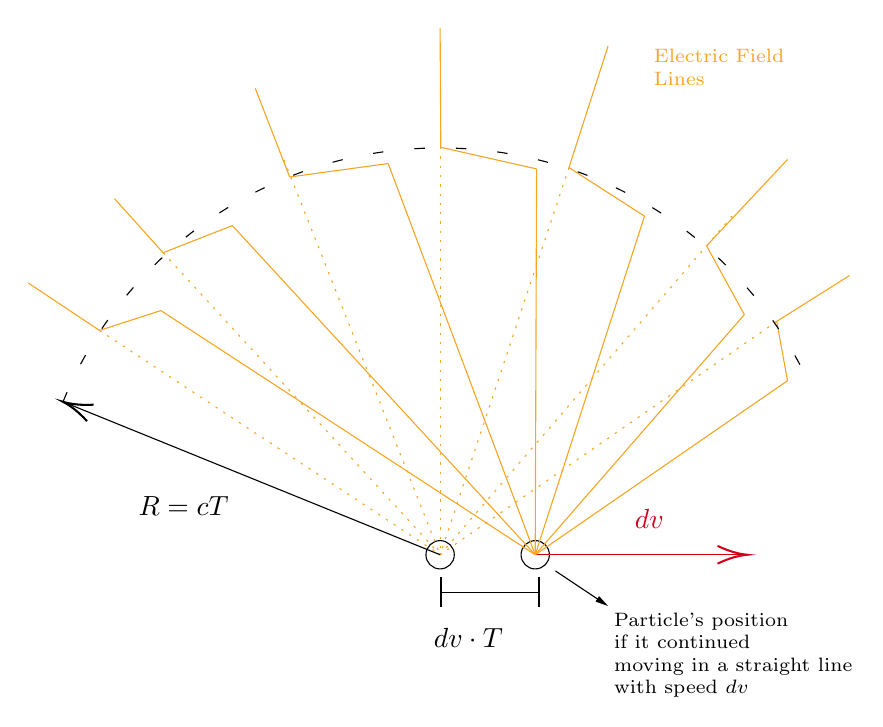
\begin{tikzpicture}[x=0.75pt,y=0.75pt,yscale=-1.3,xscale=1.3]
%uncomment if require: \path (0,643); %set diagram left start at 0, and has height of 643

%Shape: Circle [id:dp45408164622656866] 
\draw   (186,276.42) .. controls (186,273.52) and (188.35,271.17) .. (191.25,271.17) .. controls (194.15,271.17) and (196.5,273.52) .. (196.5,276.42) .. controls (196.5,279.32) and (194.15,281.67) .. (191.25,281.67) .. controls (188.35,281.67) and (186,279.32) .. (186,276.42) -- cycle ;
%Shape: Circle [id:dp9495535269700299] 
\draw   (221.25,276.42) .. controls (221.25,273.52) and (223.6,271.17) .. (226.5,271.17) .. controls (229.4,271.17) and (231.75,273.52) .. (231.75,276.42) .. controls (231.75,279.32) and (229.4,281.67) .. (226.5,281.67) .. controls (223.6,281.67) and (221.25,279.32) .. (221.25,276.42) -- cycle ;
%Straight Lines [id:da5372483043196656] 
\draw [color={rgb, 255:red, 208; green, 2; blue, 27 }  ,draw opacity=1 ]   (226.5,276.42) -- (303,276.42) ;
\draw [shift={(305,276.42)}, rotate = 180] [color={rgb, 255:red, 208; green, 2; blue, 27 }  ,draw opacity=1 ][line width=0.75]    (10.93,-3.29) .. controls (6.95,-1.4) and (3.31,-0.3) .. (0,0) .. controls (3.31,0.3) and (6.95,1.4) .. (10.93,3.29)   ;
%Straight Lines [id:da29337150782879706] 
\draw [color={rgb, 255:red, 245; green, 166; blue, 35 }  ,draw opacity=1 ] [dash pattern={on 0.84pt off 2.51pt}]  (65,193.28) -- (191.25,276.42) ;
%Straight Lines [id:da9902672557005923] 
\draw [color={rgb, 255:red, 245; green, 166; blue, 35 }  ,draw opacity=1 ] [dash pattern={on 0.84pt off 2.51pt}]  (88.6,164.48) -- (191.25,276.42) ;
%Straight Lines [id:da6726912020090494] 
\draw [color={rgb, 255:red, 245; green, 166; blue, 35 }  ,draw opacity=1 ] [dash pattern={on 0.84pt off 2.51pt}]  (133.4,130.07) -- (191.25,276.42) ;
%Straight Lines [id:da1382779799463616] 
\draw [color={rgb, 255:red, 245; green, 166; blue, 35 }  ,draw opacity=1 ] [dash pattern={on 0.84pt off 2.51pt}]  (191.25,121.92) -- (191.25,276.42) ;
%Straight Lines [id:da03673313331060535] 
\draw [color={rgb, 255:red, 245; green, 166; blue, 35 }  ,draw opacity=1 ]   (267,150.92) -- (226.5,276.42) ;
%Straight Lines [id:da22756516333460386] 
\draw [color={rgb, 255:red, 245; green, 166; blue, 35 }  ,draw opacity=1 ] [dash pattern={on 0.84pt off 2.51pt}]  (299.5,150.92) -- (191.25,276.42) ;
%Straight Lines [id:da17712209707959925] 
\draw [color={rgb, 255:red, 245; green, 166; blue, 35 }  ,draw opacity=1 ] [dash pattern={on 0.84pt off 2.51pt}]  (316,189.92) -- (191.25,276.42) ;
%Straight Lines [id:da3439378780875706] 
\draw [color={rgb, 255:red, 245; green, 166; blue, 35 }  ,draw opacity=1 ]   (343,172.92) -- (316,189.92) ;
%Straight Lines [id:da3597146623326428] 
\draw [color={rgb, 255:red, 245; green, 166; blue, 35 }  ,draw opacity=1 ]   (316,189.92) -- (320,211.92) ;
%Straight Lines [id:da2362080685290331] 
\draw [color={rgb, 255:red, 245; green, 166; blue, 35 }  ,draw opacity=1 ]   (320,129.92) -- (290,161.92) ;
%Straight Lines [id:da6285095588278771] 
\draw [color={rgb, 255:red, 245; green, 166; blue, 35 }  ,draw opacity=1 ]   (304,187.42) -- (290,161.92) ;
%Straight Lines [id:da49865556910052034] 
\draw [color={rgb, 255:red, 245; green, 166; blue, 35 }  ,draw opacity=1 ]   (253.5,87.92) -- (239,132.92) ;
%Straight Lines [id:da42581639547252403] 
\draw [color={rgb, 255:red, 245; green, 166; blue, 35 }  ,draw opacity=1 ]   (239,132.92) -- (267,150.92) ;
%Straight Lines [id:da3964515350998439] 
\draw [color={rgb, 255:red, 245; green, 166; blue, 35 }  ,draw opacity=1 ] [dash pattern={on 0.84pt off 2.51pt}]  (239,132.92) -- (191.25,276.42) ;
%Straight Lines [id:da20364150993901875] 
\draw [color={rgb, 255:red, 245; green, 166; blue, 35 }  ,draw opacity=1 ]   (320,211.92) -- (226.5,276.42) ;
%Straight Lines [id:da37251480611928045] 
\draw [color={rgb, 255:red, 245; green, 166; blue, 35 }  ,draw opacity=1 ]   (304,187.42) -- (226.5,276.42) ;
%Straight Lines [id:da4884503948352661] 
\draw [color={rgb, 255:red, 245; green, 166; blue, 35 }  ,draw opacity=1 ]   (227,133.42) -- (226.5,276.42) ;
%Straight Lines [id:da2572352246393719] 
\draw [color={rgb, 255:red, 245; green, 166; blue, 35 }  ,draw opacity=1 ]   (191.5,125.42) -- (227,133.42) ;
%Straight Lines [id:da8603805578611294] 
\draw [color={rgb, 255:red, 245; green, 166; blue, 35 }  ,draw opacity=1 ]   (191.5,125.42) -- (191.25,81.28) ;
%Straight Lines [id:da6461667950822738] 
\draw [color={rgb, 255:red, 245; green, 166; blue, 35 }  ,draw opacity=1 ]   (172,131.42) -- (226.5,276.42) ;
%Straight Lines [id:da487067822337389] 
\draw [color={rgb, 255:red, 245; green, 166; blue, 35 }  ,draw opacity=1 ]   (172,131.42) -- (135.5,136.42) ;
%Straight Lines [id:da1549395926588819] 
\draw [color={rgb, 255:red, 245; green, 166; blue, 35 }  ,draw opacity=1 ]   (122.75,103.59) -- (135.5,136.42) ;
%Straight Lines [id:da08023353090467689] 
\draw [color={rgb, 255:red, 245; green, 166; blue, 35 }  ,draw opacity=1 ]   (114.25,154.42) -- (226.5,276.42) ;
%Straight Lines [id:da5899311527256579] 
\draw [color={rgb, 255:red, 245; green, 166; blue, 35 }  ,draw opacity=1 ]   (88.6,164.48) -- (114.25,154.42) ;
'%Straight Lines [id:da249344649589599] 
\draw [color={rgb, 255:red, 245; green, 166; blue, 35 }  ,draw opacity=1 ]   (70.6,144.48) -- (88.6,164.48) ;
%Straight Lines [id:da3238263717491934] 
\draw [color={rgb, 255:red, 245; green, 166; blue, 35 }  ,draw opacity=1 ]   (87.75,185.92) -- (226.5,276.42) ;
%Straight Lines [id:da7228583033060747] 
\draw [color={rgb, 255:red, 245; green, 166; blue, 35 }  ,draw opacity=1 ]   (65,193.28) -- (87.75,185.92) ;
%Straight Lines [id:da5929533076819347] 
\draw [color={rgb, 255:red, 245; green, 166; blue, 35 }  ,draw opacity=1 ]   (38.6,175.68) -- (65,193.28) ;
%Straight Lines [id:da16203706446751953] 
\draw    (191.5,290.3) -- (227.75,290.3) ;
\draw [shift={(227.75,290.3)}, rotate = 180] [color={rgb, 255:red, 0; green, 0; blue, 0 }  ][line width=0.75]    (0,5.59) -- (0,-5.59)   ;
\draw [shift={(191.5,290.3)}, rotate = 180] [color={rgb, 255:red, 0; green, 0; blue, 0 }  ][line width=0.75]    (0,5.59) -- (0,-5.59)   ;
%Straight Lines [id:da6371275319025769] 
\draw    (234,282.42) -- (251.84,294.31) ;
\draw [shift={(253.5,295.42)}, rotate = 213.69] [fill={rgb, 255:red, 0; green, 0; blue, 0 }  ][line width=0.08]  [draw opacity=0] (4.8,-1.2) -- (0,0) -- (4.8,1.2) -- cycle    ;
%Shape: Arc [id:dp440305270368335] 
\draw  [draw opacity=0][dash pattern={on 3.75pt off 11.25pt}] (51.49,219.73) .. controls (73.9,164.55) and (128.03,125.64) .. (191.25,125.64) .. controls (252.51,125.64) and (305.24,162.18) .. (328.84,214.65) -- (191.25,276.42) -- cycle ; \draw  [dash pattern={on 3.75pt off 11.25pt}] (51.49,219.73) .. controls (73.9,164.55) and (128.03,125.64) .. (191.25,125.64) .. controls (252.51,125.64) and (305.24,162.18) .. (328.84,214.65) ;  
%Straight Lines [id:da34549181600548384] 
\draw    (191.25,276.42) -- (53.34,220.48) ;
\draw [shift={(51.49,219.73)}, rotate = 22.08] [color={rgb, 255:red, 0; green, 0; blue, 0 }  ][line width=0.75]    (10.93,-3.29) .. controls (6.95,-1.4) and (3.31,-0.3) .. (0,0) .. controls (3.31,0.3) and (6.95,1.4) .. (10.93,3.29)   ;

% Text Node
\draw (269.5,88.17) node [anchor=north west][inner sep=0.75pt]  [font=\scriptsize,color={rgb, 255:red, 245; green, 166; blue, 35 }  ,opacity=1 ] [align=left] {Electric Field\\Lines};
% Text Node
\draw (188,302.57) node [anchor=north west][inner sep=0.75pt]    {$dv\cdot T$};
% Text Node
\draw (254.75,297.17) node [anchor=north west][inner sep=0.75pt] [font = \scriptsize] [align=left] {Particle's position\\if it continued\\moving in a straight line\\with speed $\displaystyle dv$};
% Text Node
\draw (262.5,258.57) node [anchor=north west][inner sep=0.75pt]  [color={rgb, 255:red, 208; green, 2; blue, 27 }  ,opacity=1 ]  {$dv$};
% Text Node
\draw (78.5,254.07) node [anchor=north west][inner sep=0.75pt]    {$R=cT$};


\end{tikzpicture}


\caption{Variation of electric field lines due to the particle's motion. As the particle moves, the field lines adjust to its new position, generating a disturbance that propagates at the speed of light $c$}
\label{fig:nicerelativity}
\end{figure}

\ut{B.1} Note that in the disturbance zone the electric field has a component perpendicular $\vec{E}_\perp$ to the particle (not only the radial component: $\vec{E}_r$). Thus, find the value of $\dfrac{|\vec{E}_\perp|}{|\vec{E}_r|}$ for the region at an angle $\theta$ with $dv$, as a function of $a,\ T,\ \theta$, and $c$.

\ut{B.2} Knowing that $E_r$ is normally calculated by Coulomb's law, find the value of $E_\perp$ as a function of $q,\ a,\ \theta,\ R$, and $c$.

\ut{B.3} Argue that, in a region sufficiently far from the dipole, the electric field can be approximated as $E_\perp$.

\ut{B.4} Considering that the radiation flux (power emitted per unit area) in a region of space is defined as:

\[\vec{S} = \frac{1}{\mu_0} \vec{E} \times \vec{B}\]

Thus, find the flux at a region at a distance $R$ from the particle's initial position and at an angle $\theta$ from the direction of $dv$.

\ut{B.5} Show that the total power emitted due to the dipole's rotation can be expressed as:

\[P_{ele} = \frac{p^2 \Omega^4}{6\pi\epsilon_0c^3}\]

where $p = qR$ is the dipole moment of the particle system.

\parte{C}{Pulsars}

Consider for this part a neutron star that has a magnetic field at its north magnetic pole equal to $B$, radius $R$, mass $M$, and rotation period $P$. This celestial body has its magnetic axis tilted by an angle $\theta$ relative to the rotation axis, as shown in Figure \ref{fig:pulsar}.
        
    
    \begin{figure}[htpb]
        \centering
        

\tikzset{every picture/.style={line width=0.75pt}} %set default line width to 0.75pt        

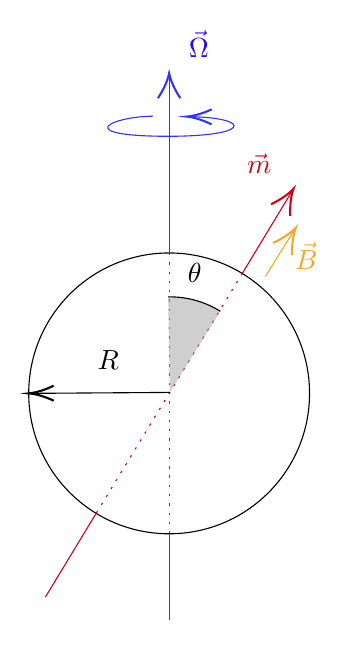
\begin{tikzpicture}[x=0.75pt,y=0.75pt,yscale=-1.1,xscale=1.1]
%uncomment if require: \path (0,643); %set diagram left start at 0, and has height of 643

%Shape: Circle [id:dp4232876725439978] 
\draw   (281,221.5) .. controls (281,187.53) and (308.53,160) .. (342.5,160) .. controls (376.47,160) and (404,187.53) .. (404,221.5) .. controls (404,255.47) and (376.47,283) .. (342.5,283) .. controls (308.53,283) and (281,255.47) .. (281,221.5) -- cycle ;
%Straight Lines [id:da8006792996850713] 
\draw [color={rgb, 255:red, 50; green, 50; blue, 250 }  ,draw opacity=1 ]   (342.5,83.28) -- (342.5,160) ;
\draw [shift={(342.5,81.28)}, rotate = 90] [color={rgb, 255:red, 50; green, 50; blue, 250 }  ,draw opacity=1 ][line width=0.75]    (10.93,-4.9) .. controls (6.95,-2.3) and (3.31,-0.67) .. (0,0) .. controls (3.31,0.67) and (6.95,2.3) .. (10.93,4.9)   ;
%Straight Lines [id:da05347487884717195] 
\draw [color={rgb, 255:red, 50; green, 50; blue, 250 }  ,draw opacity=1 ]   (342.5,283) -- (342.5,320.92) ;
%Straight Lines [id:da6868599461584712] 
\draw [color={rgb, 255:red, 50; green, 50; blue, 250 }  ,draw opacity=1 ] [dash pattern={on 0.84pt off 2.51pt}]  (342.5,160) -- (342.5,283) ;
%Straight Lines [id:da4348706602531407] 
\draw [color={rgb, 255:red, 208; green, 2; blue, 27 }  ,draw opacity=1 ]   (311,273.27) -- (288.3,310.75) ;
%Straight Lines [id:da7168654595531465] 
\draw [color={rgb, 255:red, 208; green, 2; blue, 27 }  ,draw opacity=1 ]   (395.97,133.54) -- (374.6,168.88) ;
\draw [shift={(397,131.83)}, rotate = 121.16] [color={rgb, 255:red, 208; green, 2; blue, 27 }  ,draw opacity=1 ][line width=0.75]    (10.93,-4.9) .. controls (6.95,-2.3) and (3.31,-0.67) .. (0,0) .. controls (3.31,0.67) and (6.95,2.3) .. (10.93,4.9)   ;
%Straight Lines [id:da9790784319350223] 
\draw [color={rgb, 255:red, 208; green, 2; blue, 27 }  ,draw opacity=1 ] [dash pattern={on 0.84pt off 2.51pt}]  (374.6,168.88) -- (311,273.27) ;
%Shape: Arc [id:dp2768111157212205] 
\draw  [draw opacity=0][fill={rgb, 255:red, 155; green, 155; blue, 155 }  ,fill opacity=0.48 ] (342.07,179.23) .. controls (342.31,179.23) and (342.56,179.23) .. (342.8,179.23) .. controls (350.93,179.23) and (358.51,181.54) .. (364.93,185.55) -- (342.8,221.08) -- cycle ; \draw   (342.07,179.23) .. controls (342.31,179.23) and (342.56,179.23) .. (342.8,179.23) .. controls (350.93,179.23) and (358.51,181.54) .. (364.93,185.55) ;  
%Curve Lines [id:da21075349278045352] 
\draw [color={rgb, 255:red, 50; green, 50; blue, 250 }  ,draw opacity=1 ]   (335.33,100.09) .. controls (317,100.34) and (300.19,108.55) .. (339.86,108.89) .. controls (378.73,109.21) and (379.28,100.94) .. (351.88,100.29) ;
\draw [shift={(350.17,100.26)}, rotate = 0.68] [color={rgb, 255:red, 50; green, 50; blue, 250 }  ,draw opacity=1 ][line width=0.75]    (10.93,-3.29) .. controls (6.95,-1.4) and (3.31,-0.3) .. (0,0) .. controls (3.31,0.3) and (6.95,1.4) .. (10.93,3.29)   ;
%Straight Lines [id:da3842889774147502] 
\draw    (342.8,221.08) -- (283,221.49) ;
\draw [shift={(281,221.5)}, rotate = 359.61] [color={rgb, 255:red, 0; green, 0; blue, 0 }  ][line width=0.75]    (10.93,-3.29) .. controls (6.95,-1.4) and (3.31,-0.3) .. (0,0) .. controls (3.31,0.3) and (6.95,1.4) .. (10.93,3.29)   ;
%Straight Lines [id:da830376172544915] 
\draw [color={rgb, 255:red, 245; green, 166; blue, 35 }  ,draw opacity=1 ]   (396.94,150.62) -- (384.6,170.38) ;
\draw [shift={(398,148.92)}, rotate = 121.99] [color={rgb, 255:red, 245; green, 166; blue, 35 }  ,draw opacity=1 ][line width=0.75]    (10.93,-4.9) .. controls (6.95,-2.3) and (3.31,-0.67) .. (0,0) .. controls (3.31,0.67) and (6.95,2.3) .. (10.93,4.9)   ;

% Text Node
\draw (349.6,163.48) node [anchor=north west][inner sep=0.75pt]    {$\theta $};
% Text Node
\draw (375.5,115.23) node [anchor=north west][inner sep=0.75pt]  [color={rgb, 255:red, 208; green, 2; blue, 27 }  ,opacity=1 ]  {$\vec{m}$};
% Text Node
\draw (350,61.57) node [anchor=north west][inner sep=0.75pt]  [color={rgb, 255:red, 50; green, 0; blue, 250 }  ,opacity=1 ]  {$\vec{\Omega }$};
% Text Node
\draw (310,201.4) node [anchor=north west][inner sep=0.75pt]    {$R$};
% Text Node
\draw (396.5,154.57) node [anchor=north west][inner sep=0.75pt]  [color={rgb, 255:red, 245; green, 166; blue, 35 }  ,opacity=1 ]  {$\vec{B}$};


\end{tikzpicture}

    
        \caption{Graphical scheme of the pulsar in question, the rotation axis is represented by the angular velocity vector with magnitude $\dfrac{2\pi}{P}$}
        \label{fig:pulsar}
    \end{figure}
    
    Note that in this case, the variable dipole moment is not an electric dipole, but rather a magnetic dipole. Nevertheless, a similar intuition is used to calculate the power dissipated by a magnetic dipole $m$ rotating in uniform circular motion with angular velocity $\Omega$, whose equation is presented as follows:
    
    \[P_{mag} = \frac{\mu_0}{6\pi c^3} m^2 \Omega^4\]
    
    \ut{C.1} Considering that the magnetic field in a region of space with $R \le |\vec{r}|$ is described by equation \ref{eq:magneticfield}, find the power emitted by the pulsar as a function of $B,\ R,\ \theta,\ P$ and other natural constants.
    
    Measuring the magnetic field of a distant celestial body is a complex task; however, from the relation in the previous item, it is possible to relate this physical quantity to other parameters that are easier to detect. Therefore:
    
    \ut{C.2} Considering that the pulsar has a homogeneous matter distribution, that the dissipated power comes from the rotational kinetic energy of the pulsar, and that it has a period variation rate $\dot{P}$, calculate the magnetic field $B$ at the magnetic north pole of the star.
    
    \clearpage
    \fi

    \ifsolution
    \section{Pulsars}

    \parte{A}{Let There Be Light!}
    
    \ut{A.1} For the electromagnetic wave described in the statement, it is possible to describe its electric and magnetic fields as functions of position $x$ and time $t$ such that:
    
    \[\begin{cases}
    \vec{E} = E(x,t)\hat{j} \\
    \vec{B} = B(x,t)\hat{k}
    \end{cases}\]
    
    So that:
    
    \[\nabla \times \vec{E} = \begin{vmatrix}
    \hat{i} & \hat{j} & \hat{k} \\
    \frac{\partial}{\partial x} & \frac{\partial}{\partial y} & \frac{\partial}{\partial z} \\
    0 & E(x,t) & 0
    \end{vmatrix}\]
    
    \[\frac{\partial \vec{B}}{\partial t} = \frac{\partial B(x,t)}{\partial t} \hat{k}\]
    
    Therefore, it is possible to write Maxwell's relation 3 as:
    
    \[\frac{\partial E(x,t)}{\partial x} \hat{k} - \frac{\partial E(x,t)}{\partial z} \hat{i} = - \frac{\partial B(x,t)}{\partial t} \hat{k} \]
    
    Since $E(x,t)$ does not depend on $z$, we can state that $\dfrac{\partial E(x,t)}{\partial z} = 0$. Therefore, we have:
    
    \begin{equation}
        \frac{\partial E(x,t)}{\partial x}  = - \frac{\partial B(x,t)}{\partial t}
        \label{eq:eq1maxwell}
    \end{equation}
    
    Similarly, for Maxwell's relation 4:
    
    \[\nabla \times \vec{B} = \begin{vmatrix}
    \hat{i} & \hat{j} & \hat{k} \\
    \frac{\partial}{\partial x} & \frac{\partial}{\partial y} & \frac{\partial}{\partial z} \\
    0 & 0 & B(x,t)
    \end{vmatrix} = \frac{\partial B(x,t)}{\partial y} \hat{i} - \frac{\partial B(x,t)}{\partial x} \hat{j}\]
    
    \[\frac{\partial \vec{E}}{\partial t} = \frac{\partial E(x,t)}{\partial t} \hat{j}\]
    
    Therefore, knowing that $\dfrac{\partial B(x,t)}{\partial y} = 0$, we can conclude:
    
    \begin{equation}
        \frac{\partial B(x,t)}{\partial x} = -\mu_0 \epsilon_0 \frac{\partial E(x,t)}{\partial t}
        \label{eq:eq2maxwell}
    \end{equation}
    
    We will use the fact that $E(x,t)$ and $B(x,t)$ are smooth functions\footnote{That is, functions of class $C^2$.}, so it is possible to apply Fubini's theorem, according to which, given $f(x,y): D \rightarrow \RR$ a $C^2$ function:
    
    \[\frac{\partial^2 f(x,y)}{\partial x \partial y} = \frac{\partial^2 f(x,y)}{\partial y \partial x}\]
    
    Thus, taking the partial derivative with respect to time of equation \ref{eq:eq1maxwell} and the partial derivative with respect to $x$ of equation \ref{eq:eq2maxwell}, we get:
    
    \[\begin{cases}
    \dfrac{\partial^2 E(x,t)}{\partial t \partial x} = -\dfrac{\partial^2 B(x,t)}{\partial t^2} \\
    
    \\
    
    \dfrac{\partial^2 B(x,t)}{\partial x^2} = - \mu_0 \epsilon_0 \dfrac{\partial^2 E(x,t)}{\partial x \partial t}
    \end{cases}\]
    
    Equating the partial derivatives of $E(x,t)$ by Fubini's theorem, we have:
    
    \[\therefore \frac{\partial ^2 B(x,t)}{\partial x^2} = \mu_0 \epsilon_0\frac{\partial^2 B(x,t)}{\partial t^2}\]
    
    Therefore, from the fundamental wave equation, we can conclude that the propagation speed of the electromagnetic wave is always $c = \dfrac{1}{\sqrt{\mu_0 \epsilon_0}}$.
    
    \ut{A.2} Note that for this type of wave function (the same relation holds for $B(x,t)$):
    
    \[\frac{\partial E}{\partial x} = -\frac{1}{c} \frac{\partial E}{\partial t}\]
    
    Thus, from equations \ref{eq:eq1maxwell} and \ref{eq:eq2maxwell}, the maxima and minima of the magnetic and electric field oscillations must occur simultaneously\footnote{If one derivative is zero, the other must also be zero.}. This implies that the functions must be coherent with each other; hence we conclude that $k_1 = k_2,\ \omega_1 = \omega_2$, and $\phi_1 = \phi_2$ (for simplicity, we assume $\phi_1 = 0$).
    
    \ut{A.3} From equation \ref{eq:eq1maxwell}:
    
    \[E_0 k \cos(kx-\omega t) = B_0 \omega \cos(kx-\omega t)\]
    
    \[\therefore E_0 = \frac{\omega}{k} B_0\]
    
    Since $\omega = 2\pi f$ and $k = \dfrac{2\pi}{\lambda}$, it follows that $\dfrac{\omega}{k} = \lambda f = c$:
    
    \[\therefore E_0 = c B_0\]
    
    Therefore, we can see that $|\vec{E}(x,t)| = |\vec{B}(x,t)|,\ \forall x,t \in \RR$.
    
    \parte{B}{Variable Dipole}

    \ut{B.1} Consider figure \ref{fig:resolution}, which addresses the situation presented, taking into account the problem conditions.

    \begin{figure}[htpb]
        \centering
        

\tikzset{every picture/.style={line width=0.75pt}} %set default line width to 0.75pt        

\begin{tikzpicture}[x=0.75pt,y=0.75pt,yscale=-1,xscale=1]
%uncomment if require: \path (0,643); %set diagram left start at 0, and has height of 643

%Straight Lines [id:da9447788484778064] 
\draw  [dash pattern={on 4.5pt off 4.5pt}]  (213.86,324.34) -- (383,324.34) ;
%Shape: Circle [id:dp6457607875494435] 
\draw   (207.09,324.34) .. controls (207.09,320.61) and (210.12,317.58) .. (213.86,317.58) .. controls (217.59,317.58) and (220.62,320.61) .. (220.62,324.34) .. controls (220.62,328.08) and (217.59,331.11) .. (213.86,331.11) .. controls (210.12,331.11) and (207.09,328.08) .. (207.09,324.34) -- cycle ;
%Shape: Circle [id:dp3802923013140629] 
\draw   (341.19,324.34) .. controls (341.19,320.61) and (344.22,317.58) .. (347.95,317.58) .. controls (351.69,317.58) and (354.72,320.61) .. (354.72,324.34) .. controls (354.72,328.08) and (351.69,331.11) .. (347.95,331.11) .. controls (344.22,331.11) and (341.19,328.08) .. (341.19,324.34) -- cycle ;
%Straight Lines [id:da32720331603233177] 
\draw    (407.95,102.37) -- (456.45,200.41) ;
%Straight Lines [id:da38591544870374306] 
\draw    (456.45,200.41) -- (347.95,324.34) ;
%Straight Lines [id:da5384320273764838] 
\draw    (478.45,25.81) -- (407.95,102.37) ;
%Straight Lines [id:da09699531355685598] 
\draw  [dash pattern={on 0.84pt off 2.51pt}]  (407.95,102.37) -- (213.86,324.34) ;
%Straight Lines [id:da7734376017399689] 
\draw    (360.89,160.01) -- (430.06,226.98) ;
\draw [shift={(431.5,228.37)}, rotate = 224.07] [color={rgb, 255:red, 0; green, 0; blue, 0 }  ][line width=0.75]    (10.93,-3.29) .. controls (6.95,-1.4) and (3.31,-0.3) .. (0,0) .. controls (3.31,0.3) and (6.95,1.4) .. (10.93,3.29)   ;
\draw [shift={(359.45,158.62)}, rotate = 44.07] [color={rgb, 255:red, 0; green, 0; blue, 0 }  ][line width=0.75]    (10.93,-3.29) .. controls (6.95,-1.4) and (3.31,-0.3) .. (0,0) .. controls (3.31,0.3) and (6.95,1.4) .. (10.93,3.29)   ;
%Shape: Pie [id:dp6297157187835885] 
\draw   (368.95,300.99) .. controls (375.11,306.67) and (379.01,314.81) .. (379.14,323.88) -- (347.95,324.34) -- cycle ;
%Shape: Pie [id:dp5912527105329268] 
\draw   (225.08,311.86) .. controls (228.37,314.9) and (230.45,319.25) .. (230.52,324.09) -- (213.86,324.34) -- cycle ;
%Curve Lines [id:da3441369411223425] 
\draw    (400,101.71) .. controls (360.86,117.23) and (360.67,57.91) .. (296.97,80.96) ;
\draw [shift={(296,81.31)}, rotate = 339.64] [color={rgb, 255:red, 0; green, 0; blue, 0 }  ][line width=0.75]    (10.93,-3.29) .. controls (6.95,-1.4) and (3.31,-0.3) .. (0,0) .. controls (3.31,0.3) and (6.95,1.4) .. (10.93,3.29)   ;
%Straight Lines [id:da5862423716495089] 
\draw    (482.72,176.32) -- (461.73,201.54) ;
\draw [shift={(460.45,203.08)}, rotate = 309.77] [color={rgb, 255:red, 0; green, 0; blue, 0 }  ][line width=0.75]    (8.74,-2.63) .. controls (5.56,-1.12) and (2.65,-0.24) .. (0,0) .. controls (2.65,0.24) and (5.56,1.12) .. (8.74,2.63)   ;
\draw [shift={(484,174.78)}, rotate = 129.77] [color={rgb, 255:red, 0; green, 0; blue, 0 }  ][line width=0.75]    (8.74,-2.63) .. controls (5.56,-1.12) and (2.65,-0.24) .. (0,0) .. controls (2.65,0.24) and (5.56,1.12) .. (8.74,2.63)   ;
%Straight Lines [id:da6108319967738429] 
\draw  [dash pattern={on 0.84pt off 2.51pt}]  (407.95,102.37) -- (480,172.12) ;
%Curve Lines [id:da3362794545077916] 
\draw    (458,208.71) .. controls (483.07,225.58) and (447.06,246.33) .. (501.65,261.3) ;
\draw [shift={(503.33,261.75)}, rotate = 194.74] [color={rgb, 255:red, 0; green, 0; blue, 0 }  ][line width=0.75]    (10.93,-3.29) .. controls (6.95,-1.4) and (3.31,-0.3) .. (0,0) .. controls (3.31,0.3) and (6.95,1.4) .. (10.93,3.29)   ;

% Text Node
\draw (254.45,342.81) node [anchor=north west][inner sep=0.75pt]    {$dv\cdotp T$};
% Text Node
\draw (380,297.07) node [anchor=north west][inner sep=0.75pt]    {$\theta $};
% Text Node
\draw (210.5,292.57) node [anchor=north west][inner sep=0.75pt]    {$\theta $};
% Text Node
\draw (355.04,170.1) node [anchor=north west][inner sep=0.75pt]  [rotate=-42.46]  {$dv\cdotp T\cdotp \sin( \theta )$};
% Text Node
\draw (227.33,74.33) node [anchor=north west][inner sep=0.75pt]   [align=left] {Disturbance's\\beginning};
% Text Node
\draw (272.86,223.99) node [anchor=north west][inner sep=0.75pt]  [rotate=-310.08]  {$c\cdot T$};
% Text Node
\draw (393.53,280.66) node [anchor=north west][inner sep=0.75pt]  [rotate=-310.08]  {$c\cdot ( T-dt)$};
% Text Node
\draw (469.03,206.68) node [anchor=north west][inner sep=0.75pt]  [rotate=-309.19]  {$c\cdot dt$};
% Text Node
\draw (507.33,242.33) node [anchor=north west][inner sep=0.75pt]   [align=left] {Disturbance's\\ending};


\end{tikzpicture}

    
        \caption{Variation of the electric field lines due to the acceleration of a charged particle}
        \label{fig:resolution}
    \end{figure}
    
    Note that, in the perturbation region, it is possible to compare the intensities of the radial and transverse components of the electric field using the distances in the formed triangle, where $E_r$ is proportional to $E_\perp$ just as $c \cdot dt$ is proportional to $dv \cdot T \cdot \sin(\theta)$. Therefore:
    
    \[\frac{E_\perp}{E_r} = \frac{dv \cdot T \cdot \sin(\theta)}{c \cdot dt} = \frac{a T \sin(\theta)}{c}\]
    
    \ut{B.2} Knowing that $E_r = \dfrac{kq}{r^2}$, we have:
    
    \[E_\perp = \frac{k q a T \sin(\theta)}{c r^2}\]
    
    Since the distance $r$ from the point of field application is $r = c \cdot T \implies T = \dfrac{r}{c}$, as stated in the problem, it is possible to write $E_\perp$ as:
    
    \[E_\perp = \frac{k q a \sin(\theta)}{c^2 r}\]
    
    \ut{B.3} Note the convenient fact that $E_\perp \propto \dfrac{1}{r}$ and not $\dfrac{1}{r^2}$ as $E_r$, so that, for a region sufficiently far from the dipole, we can assert that $E_\perp >> E_r$ and therefore it corresponds to the total electric field in the region (allowing us to neglect the radial component). Even considering the particle that is not accelerated (the one with charge $-q$), the electric field from it is also proportional to $r^{-2}$, so the only "relevant" component at large distances from the dipole is the transverse one.
    
    \ut{B.4} Since this is an electromagnetic wave, the magnetic field is perpendicular to the electric field with magnitude such that $B = E / c$, therefore the radiation flux can be written as:
    
    \[S = \frac{1}{\mu_0 c} E^2 = \frac{k^2 q^2 a^2 \sin^2(\theta)}{\mu_0 c^5 r^2}\]
    
    \ut{B.5} In order to find the total power emitted throughout space, one just needs to integrate this result over all surface elements. For an interval $[\theta, \theta + d\theta]$, there exists a spherical region of area $2\pi r^2 \sin(\theta) d\theta$, so the integral becomes:
    
    \[P = \oint S dA = \int_0^\pi S(2 \pi r^2 \sin(\theta)) d\theta = \frac{2 \pi k^2 q^2 a^2}{\mu_0 c^5} \int_0^\pi \sin^3(\theta) d\theta\]
    
    Note that $\sin^3(\theta) d\theta = \sin^2(\theta) \cdot (\sin(\theta) d\theta) = (1 - \cos^2(\theta)) (-d\cos(\theta))$, therefore:
    
    \[\int_0^\pi \sin^3(\theta) d\theta = \int_{-1}^{1} 1 - x^2 dx = \frac{4}{3}\]
    
    \[\therefore P = \frac{8 \pi k^2 q^2 a^2}{3 \mu_0 c^5}\]
    
    Substituting $k = \dfrac{1}{4 \pi \epsilon_0}$, the particle's acceleration $a = \Omega^2 R$, and the particle's charge $q = \dfrac{p}{R}$:
    
    \[P = \frac{1}{16 \pi^2 \epsilon_0^2} \frac{p^2}{R^2} \frac{8 \pi \Omega^4 R^2}{3 \mu_0 c^5} = \frac{p^2 \Omega^4}{6 \pi \epsilon_0^2 \mu_0 c^5}\]
    
    Since $\mu_0 \epsilon_0 = c^{-2}$:
    
    \[P_{ele} = \frac{p^2 \Omega^4}{6 \pi \epsilon_0 c^3}\]
    
    \parte{C}{Pulsars}
    
    \ut{C.1} The magnetic north pole is the one where $\theta$ in equation \ref{eq:magneticfield} equals $0$, so that:
    
    \[B = \frac{\mu_0 m}{2 \pi R^3}\]
    
    Therefore, its magnetic dipole moment is $m = \dfrac{2 \pi}{\mu_0} B R^3$. Note, however, that the pulsar's magnetic dipole moment is inclined at an angle $\theta$, so we can decompose it into two moment components: one parallel to the rotation axis and one perpendicular, which rotates in uniform circular motion with period $P$. Only this last component is responsible for dissipating energy, so the effective dissipating moment is $m \sin(\theta)$. Thus, the dissipated power can be calculated as:
    
    \[P_{mag} = \frac{\mu_0}{6 \pi c^3} \left( \frac{2 \pi}{\mu_0} B R^3 \sin(\theta) \right)^2 \left( \frac{2 \pi}{P} \right)^4\]
    
    \[P_{mag} = \frac{\mu_0}{6 \pi c^3} \frac{4 \pi^2}{\mu_0^2} B^2 R^6 \sin^2(\theta) \frac{16 \pi^4}{P^4} = \frac{32 \pi^5 B^2 R^6 \sin^2(\theta)}{3 \mu_0 c^3 P^4}\]
    
    \ut{C.2} The rotational kinetic energy of the pulsar is $K = \dfrac{1}{2} I \Omega^2$, where $I = \dfrac{2}{5} M R^2$ is its moment of inertia, so that:
    
    \[K = \frac{8 \pi^2 M R^2}{5 P^2}\]
    
    \[\therefore \frac{dK}{dt} = -\frac{8 \pi^2 M R^2}{5 P^3} \dot{P}\]
    
    Equating the values (and ignoring the sign, which only indicates energy loss), we obtain:

    \[\frac{8\pi^2MR^2}{5P^3}\dot{P}=\frac{32\pi^5B^2R^6\sin^2(\theta)}{3\mu_0c^3P^4}\]
    
    \[B = \frac{c}{2\pi R^2 \sin(\theta)}\sqrt{\frac{3\mu_0cMP\dot{P}}{5\pi }}\]
	
	
	
	\clearpage

	\fi
	
\end{document}
